\documentclass[12pt]{jbook}
% shuron.sty の漢字コードに注意
\usepackage{fancyhd,shuron}
\usepackage{graphics}
\usepackage[dvipdfm]{graphicx}
\usepackage{epsfig}
\usepackage{tabularx}
\usepackage{chapterbib}
\usepackage{makeidx}
\usepackage{amssymb}
\usepackage{url}
\usepackage{slashbox}

\makeatletter
\def\thefootnote{\ifnum\c@footnote>\z@\leavevmode\lower.5ex%
    \hbox{$^{*\@arabic\c@footnote}$}\fi}
\makeatother

\makeindex

% http://www.lab2.kuis.kyoto-u.ac.jp/~okita/etc/#0011
%%% jdummy.def
%
\DeclareRelationFont{JY1}{mc}{it}{}{OT1}{cmr}{it}{}
\DeclareRelationFont{JT1}{mc}{it}{}{OT1}{cmr}{it}{}
\DeclareFontShape{JY1}{mc}{m}{it}{<5> <6> <7> <8> <9> <10> sgen*min
    <10.95><12><14.4><17.28><20.74><24.88> min10
    <-> min10}{}
\DeclareFontShape{JT1}{mc}{m}{it}{<5> <6> <7> <8> <9> <10> sgen*tmin
    <10.95><12><14.4><17.28><20.74><24.88> tmin10
    <-> tmin10}{}
\DeclareRelationFont{JY1}{mc}{sl}{}{OT1}{cmr}{sl}{}
\DeclareRelationFont{JT1}{mc}{sl}{}{OT1}{cmr}{sl}{}
\DeclareFontShape{JY1}{mc}{m}{sl}{<5> <6> <7> <8> <9> <10> sgen*min
    <10.95><12><14.4><17.28><20.74><24.88> min10
    <-> min10}{}
\DeclareFontShape{JT1}{mc}{m}{sl}{<5> <6> <7> <8> <9> <10> sgen*tmin
    <10.95><12><14.4><17.28><20.74><24.88> tmin10
    <-> tmin10}{}
\DeclareRelationFont{JY1}{mc}{sc}{}{OT1}{cmr}{sc}{}
\DeclareRelationFont{JT1}{mc}{sc}{}{OT1}{cmr}{sc}{}
\DeclareFontShape{JY1}{mc}{m}{sc}{<5> <6> <7> <8> <9> <10> sgen*min
    <10.95><12><14.4><17.28><20.74><24.88> min10
    <-> min10}{}
\DeclareFontShape{JT1}{mc}{m}{sc}{<5> <6> <7> <8> <9> <10> sgen*tmin
    <10.95><12><14.4><17.28><20.74><24.88> tmin10
    <-> tmin10}{}
\DeclareRelationFont{JY1}{gt}{it}{}{OT1}{cmbx}{it}{}
\DeclareRelationFont{JT1}{gt}{it}{}{OT1}{cmbx}{it}{}
\DeclareFontShape{JY1}{mc}{bx}{it}{<5> <6> <7> <8> <9> <10> sgen*goth
    <10.95><12><14.4><17.28><20.74><24.88> goth10
    <-> goth10}{}
\DeclareFontShape{JT1}{mc}{bx}{it}{<5> <6> <7> <8> <9> <10> sgen*tgoth
    <10.95><12><14.4><17.28><20.74><24.88> tgoth10
    <-> tgoth10}{}
\DeclareRelationFont{JY1}{gt}{sl}{}{OT1}{cmbx}{sl}{}
\DeclareRelationFont{JT1}{gt}{sl}{}{OT1}{cmbx}{sl}{}
\DeclareFontShape{JY1}{mc}{bx}{sl}{<5> <6> <7> <8> <9> <10> sgen*goth
    <10.95><12><14.4><17.28><20.74><24.88> goth10
    <-> goth10}{}
\DeclareFontShape{JT1}{mc}{bx}{sl}{<5> <6> <7> <8> <9> <10> sgen*tgoth
    <10.95><12><14.4><17.28><20.74><24.88> tgoth10
    <-> tgoth10}{}
\DeclareRelationFont{JY1}{gt}{sc}{}{OT1}{cmbx}{sc}{}
\DeclareRelationFont{JT1}{gt}{sc}{}{OT1}{cmbx}{sc}{}
\DeclareFontShape{JY1}{mc}{bx}{sc}{<5> <6> <7> <8> <9> <10> sgen*goth
    <10.95><12><14.4><17.28><20.74><24.88> goth10
    <-> goth10}{}
\DeclareFontShape{JT1}{mc}{bx}{sc}{<5> <6> <7> <8> <9> <10> sgen*tgoth
    <10.95><12><14.4><17.28><20.74><24.88> tgoth10
    <-> tgoth10}{}
\DeclareRelationFont{JY1}{gt}{it}{}{OT1}{cmr}{it}{}
\DeclareRelationFont{JT1}{gt}{it}{}{OT1}{cmr}{it}{}
\DeclareFontShape{JY1}{gt}{m}{it}{<5> <6> <7> <8> <9> <10> sgen*goth
    <10.95><12><14.4><17.28><20.74><24.88> goth10
    <-> goth10}{}
\DeclareFontShape{JT1}{gt}{m}{it}{<5> <6> <7> <8> <9> <10> sgen*tgoth
    <10.95><12><14.4><17.28><20.74><24.88> tgoth10
    <-> tgoth10}{}
\endinput
%%%% end of jdummy.def


\begin{document}
\setcounter{page}{0}
\thispagestyle{empty}

\noindent

\includegraphics[height=2.0cm]{img/Lissajous_UEC_logo.eps}\\
\begin{tabular}{c}
{\Large 平成XX年度 修士論文}				\\
\end{tabular}

\vspace{2.5cm}

\begin{center}
\LARGE \bf 修論タイトル\\
%\vspace{4mm}
\end{center}

\vspace{1.5cm} 

\LARGE
\begin{flushright}
電気通信大学 大学院 ○○研究科\\
××専攻\\
1234567  名前\\

\vspace{1.6zh}

{\def\arraystretch{0.6}
\begin{tabular}{rll@{}}
指導教官	& ○○ ○○& 教授	\\
		& ○○ ○○& 教授	\\
		& ○○ ○○& 教授\\
							\\
提出日	& \multicolumn{2}{c@{}}{平成XX年1月30日}	\\
\end{tabular}
}
\end{flushright}
\normalsize
\newpage

\thispagestyle{empty}

\noindent
\begin{center}
\LARGE \bf 概要\\
\end{center}

\vspace{1.0cm} 
{\small
概要(アブストラクト)は章とせず、以下の内容を1ページに要領良くまとめる.

\begin{itemize}
\setlength{\itemsep}{-2mm}
\item 研究の背景(学術的、社会的)
\item 目的
\item 方法
\item 結論
\end{itemize}

あいうえお かきくけこ さしすせそ たちつてと
あいうえお かきくけこ さしすせそ たちつてと
あいうえお かきくけこ さしすせそ たちつてと
あいうえお かきくけこ さしすせそ たちつてと
あいうえお かきくけこ さしすせそ たちつてと
あいうえお かきくけこ さしすせそ たちつてと
あいうえお かきくけこ さしすせそ たちつてと
あいうえお かきくけこ さしすせそ たちつてと

なにぬねの はひふへほ まみむめも やいゆえよ
なにぬねの はひふへほ まみむめも やいゆえよ
なにぬねの はひふへほ まみむめも やいゆえよ
なにぬねの はひふへほ まみむめも やいゆえよ
なにぬねの はひふへほ まみむめも やいゆえよ
なにぬねの はひふへほ まみむめも やいゆえよ
なにぬねの はひふへほ まみむめも やいゆえよ
なにぬねの はひふへほ まみむめも やいゆえよ
なにぬねの はひふへほ まみむめも やいゆえよ
なにぬねの はひふへほ まみむめも やいゆえよ

わをん わをん わをん わをん わをん わをん わをん
わをん わをん わをん わをん わをん わをん わをん
わをん わをん わをん わをん わをん わをん わをん
わをん わをん わをん わをん わをん わをん わをん
わをん わをん わをん わをん わをん わをん わをん
わをん わをん わをん わをん わをん わをん わをん

な、研究を行った.
}
\normalsize
\newpage


\setcounter{page}{1}

% 目次
\tableofcontents
% 図目次
\listoffigures
% 表目次
\listoftables

% 論文本体
%序論背景と目的
\chapter{序論}\label{chap:introduction}

\section{背景}
インターネットを悪事に利用する輩は減るどころか,ますます増えつつある.
彼らは,さまざまな手法で悪事を行いつつあるため,それに対する対策を検討する
ネットワークセキュリティの重要性が増しつつある\cite{web-kinme:2016}.
そんな中,

\section{本研究の目的}

本研究の目的は,〜
本研究の目的は,〜〜〜〜〜〜
本研究の目的は,〜〜〜〜〜〜〜〜〜〜〜〜〜〜〜〜
本研究の目的は,〜〜〜〜〜〜〜〜〜〜〜〜〜〜〜〜
本研究の目的は,〜〜〜〜〜〜〜〜〜〜〜〜〜〜〜〜
本研究の目的は,〜〜〜〜〜〜〜〜〜〜〜〜〜〜〜〜
本研究の目的は,〜〜〜〜〜〜〜〜〜〜〜〜〜〜〜〜
本研究の目的は,〜〜〜〜〜〜〜〜〜〜〜〜〜〜〜〜
本研究の目的は,〜〜〜〜〜〜〜〜〜〜〜〜〜〜〜〜
本研究の目的は,〜〜〜〜〜〜〜〜〜〜〜〜〜〜〜〜
本研究の目的は,〜〜〜〜〜〜〜〜〜〜〜〜〜〜〜〜
本研究の目的は,〜〜〜〜〜〜〜〜〜〜〜〜〜〜〜〜
本研究の目的は,〜〜〜〜〜〜〜〜〜〜〜〜〜〜〜〜
本研究の目的は,〜〜〜〜〜〜〜〜〜〜〜〜〜〜〜〜
本研究の目的は,〜〜〜〜〜〜〜〜〜〜〜〜〜〜〜〜

\subsection{本研究の真の目的}
\label{subsec:ura}

本研究の真の目的は,〜〜〜〜〜〜〜〜〜〜〜〜〜〜〜〜
本研究の真の目的は,本研究の真の目的は,
本研究の真の目的は,本研究の真の目的は,本研究の真の目的は,
本研究の真の目的は,本研究の真の目的は,本研究の真の目的は,本研究の真の目的は,

\subsubsection{本研究の裏の目的}

いいねえ\cite{kasama:2011}
これもいいねぇ\cite{matsunaka:2013}
あーっと,これが一番だな\cite{Deterding:2011}.
これはきっちり目を通しておくこと.\cite{IPA}

\newpage

\section{論文の構成}
本論文は以下の章により構成される.\\

第 \ref{chap:introduction} 章 序論では,〜に関する話をし,\
第 \ref{chap:relatedwork} 章 関連研究の章では,前章で述べた問題点に
対する既存の製品や研究の取り組みを紹介する.またそれにともない,どのような
手法が対策として用いられているかを整理する.
第 \ref{chap:system} 章 システムでは,本研究で開発したシステムに関する原理と詳細説明を行う.第 \ref{chap:results} 章 結果では,なんらかの結果について報告する.
第 \ref{chap:discussion} 章 考察では,これまでの取り組みと得られた結果から,
本研究の成果と各結果に対する考察,ならびに今後の課題について考察する.\\
第 \ref{chap:conclusion} 章 結論で本研究について総括する.\\

\newpage


%関連研究
\chapter{関連研究}\label{chap:relatedwork}

こんなんのもありまっせ.
\ref{chap:introduction}章にも書きましたぜ.

\section{Aの関連研究}
\label{sec:relatedworkA}

\ref{subsec:ura}節に、本研究の真の目的を書いたが、その理由はこの関連研究にある.

\newpage

%システム
\chapter{システム}\label{chap:system}

どうなの、こうなの

\begin{figure}[th]
\begin{center}

\epsfig{file=img/Lissajous_UEC_logo.eps,scale=0.50}
\caption{リサージュ図形}
\end{center}
\label{fig:lissajous}
\end{figure}


\newpage


%結果
\chapter{結果}\label{chap:results}

こんなん結果でましたけど、どないでっしゃろ?

\begin{figure}[ht]
\begin{center}
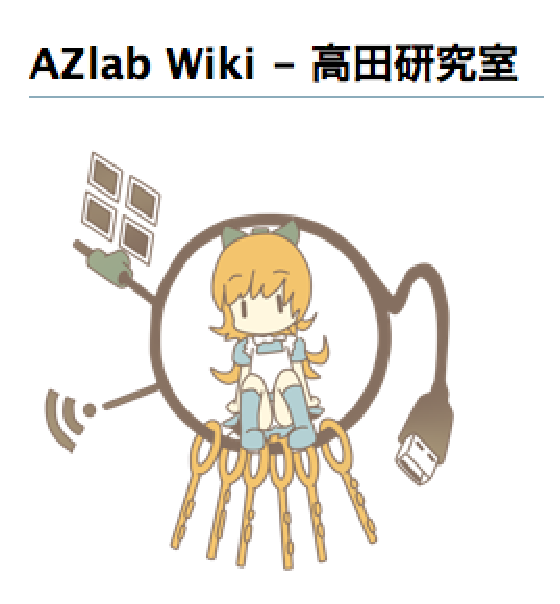
\includegraphics[scale=1.0]{img/azlabMark.eps}
\caption{our lab's web page}
\label{fig:azweb}
\end{center}
\end{figure}

図\ref{fig:azweb}は、国分君作のシンボルマーク

\newpage


%考察
\chapter{考察}\label{chap:discussion}

\section{あーだこーだの考察}\label{sec:disc1}

\subsection{あーだの考察}\label{subsec:disc2}

\begin{table}[th]
\begin{center}
\caption{なんのかんの表}
\label{tbl:hyou}
\vspace{4mm}
\begin{tabular}{l||c|r}
\hline
品目 & たて & よこ \\
\hline \hline
あれ & 1cm & 2cm \\
これ & 1.22cm & 2.87cm \\
\hline
\end{tabular}
\end{center}
\end{table}

いろいろ考えた。
あーだーこーだー あーだーこーだー あーだーこーだー あーだーこーだー
あーだーこーだー あーだーこーだー あーだーこーだー あーだーこーだー
あーだーこーだー あーだーこーだー あーだーこーだー あーだーこーだー
あーだーこーだー あーだーこーだー あーだーこーだー あーだーこーだー
あーだーこーだー あーだーこーだー あーだーこーだー あーだーこーだー
あーだーこーだー あーだーこーだー あーだーこーだー あーだーこーだー
あーだーこーだー あーだーこーだー あーだーこーだー あーだーこーだー
あーだーこーだー あーだーこーだー あーだーこーだー あーだーこーだー
あーだーこーだー あーだーこーだー あーだーこーだー あーだーこーだー
あーだーこーだー あーだーこーだー あーだーこーだー あーだーこーだー
あーだーこーだー あーだーこーだー あーだーこーだー あーだーこーだー
あーだーこーだー あーだーこーだー あーだーこーだー あーだーこーだー
あーだーこーだー あーだーこーだー あーだーこーだー あーだーこーだー
あーだーこーだー あーだーこーだー あーだーこーだー あーだーこーだー
あーだーこーだー あーだーこーだー あーだーこーだー あーだーこーだー
あーだーこーだー あーだーこーだー
あーだーこーだー あーだーこーだー あーだーこーだー あーだーこーだー
あーだーこーだー あーだーこーだー あーだーこーだー あーだーこーだー
あーだーこーだー あーだーこーだー あーだーこーだー あーだーこーだー

で、これまでの考察をまとめたのが表\ref{tbl:hyou}である.

\newpage


%結論
\chapter{結論}\label{chap:conclusion}

\newpage

%謝辞
\begin{ackn}{}

感謝します.
父上,母上,家族のみんなー
先生、研究室の諸先輩方、そして同期のみんなー

\end{ackn}{}
\newpage
% LocalWords:  ackn

%参考文献
\begin{thebibliography}{99}

\bibitem{kinme:2016}サイト名:WEBページタイトル,入手先〈\url{http://kinmemodoki.net}(参照2016-01-16).

\bibitem{kasama:2011} 笠間 貴弘,井上 大介,衛藤 将史,中里 純二,中尾 康二:ドライブ・バイ・ダウンロード攻撃対策フレームワークの提案,コンピュータセキュリティシンポジウム2011 論文集,Vol.2011,No.3,pp.780-785(2011).

\bibitem{matsunaka:2013}T.Matsunaka, J.Urakawa and A.Kubota:Detecting and Preventing Drive-by Download Attack via Participative Monitoring of the Web, {\it Proc. of 8th Asia Joint Conference on Information Security} ({\it AsiaJCIS2013}), pp.48-55, IEEE(2013).

\bibitem{Deterding:2011}Sebastian Deterding, Miguel Sicart, Lennart Nacke, Kenton O’Hara, and Dan Dixon:Gamification. using game-design elements in non-gaming contexts,{\it Proc. CHI ’11 Extended Abstracts on Human Factors in Computing Systems}({\it CHI EA’11}), pp.2425-2428, ACM(2011).

\bibitem{IPA}情報処理推進機構(IPA):ニューヨークだより 米国における「ゲーミフィケーション」の動向,入手先〈\url{http://www.ipa.go.jp/files/000006076.pdf}〉\\(参照2016-02-24).

\bibitem{swarm}Foursquare:swarm,入手先〈\url{https://www.swarmapp.com/}〉(参照2016-02-24).

\bibitem{PS3}Sony Computer Entertainment:トロフィー機能 PlayStation3 ユーザーズガイド,入手先〈\url{http://manuals.playstation.net/document/jp/ps3/current/trophy/trophy.html}〉(参照2016-02-24).

\end{thebibliography}


% 付録
%\input{appendix}

%\addcontentsline{toc}{chapter}{索引}
%\printindex

\end{document}
